\documentclass[11pt,twoside]{article}
%\documentclass[10pt,twoside,twocolumn]{article}
\usepackage[english]{babel}
\usepackage{times,subeqnarray}
\usepackage{url}
% following is for pdflatex vs. old(dvi) latex
\newif\myifpdf
\ifx\pdfoutput\undefined
%  \pdffalse           % we are not running PDFLaTeX
   \usepackage[dvips]{graphicx}
\else
   \pdfoutput=1        % we are running PDFLaTeX
%  \pdftrue
   \usepackage[pdftex]{graphicx}
\fi
%\usepackage{apatitlepages}
% if you want to be more fully apa-style for submission, then use this
%\usepackage{setspace,psypub,ulem}
%\usepackage{setspace} % must come before psypub
%\usepackage{psypub}
%\usepackage{psydraft}
%\usepackage{one-in-margins}  % use instead of psydraft for one-in-margs
%\usepackage{apa}       % apa must come last
% using latex2e as standard, use the following for latex209
% \documentstyle [times,11pt,twoside,subeqnarray,psydraft,apa,epsf]{article}
%\input netsym

% tell pdflatex to prefer .pdf files over .png files!!
\myifpdf
  \DeclareGraphicsExtensions{.pdf,.eps,.png,.jpg,.mps,.tif}
\fi

% science-specific stuff:
\usepackage{scicite}

\oddsidemargin 0pt
\evensidemargin 0pt
\textwidth 6.5in
\headheight 12pt
\headsep .5in
\topmargin -.75in
%\setlength\footheight{.25in}
\footskip .75in
\textheight 9in

\renewcommand{\topfraction}{0.95}
\renewcommand{\bottomfraction}{0.95}
\renewcommand{\textfraction}{0.05}
\renewcommand{\textfraction}{0.1}
\renewcommand{\floatpagefraction}{0.95} % limits blank space on float page
\renewcommand{\dbltopfraction}{0.95}
\renewcommand{\dblfloatpagefraction}{0.95} % limits blank space on float page

\newenvironment{sciabstract}{%
\begin{quote} \bf}
{\end{quote}}

\renewcommand\refname{References and Notes}

\newcounter{lastnote}
\newenvironment{scilastnote}{%
\setcounter{lastnote}{\value{enumiv}}%
\addtocounter{lastnote}{+1}%
\begin{list}%
{\arabic{lastnote}.}
{\setlength{\leftmargin}{.22in}}
{\setlength{\labelsep}{.5em}}}
{\end{list}}



% use 0 for psypub format 
\parskip 2pt
% for double-spacing, determines spacing 
%\doublespacing
%\setstretch{1.7}

\columnsep .25in   % 3/8 in column separation

\def\myheading{ Learning to Infer Causal Structure over Time }

% no twoside for pure apa style, use \markright with heading only
\pagestyle{myheadings}
\markboth{\hspace{.5in} \myheading \hfill}{\hfill O'Reilly et al \hspace{.5in}}

\title{Learning to Infer Causal Structure over Time}

\author{
Randall C. O'Reilly$^{1\dagger}$, co-authors..\\
\\
\normalsize{$^{1}$  Department of Psychology and Neuroscience\\
  University of Colorado Boulder} \\
\\
\small{$^\dagger$To whom correspondence should be addressed;
  email: randy.oreilly@colorado.edu}\\
}

\date{}

\begin{document}

\sloppy
\raggedbottom
\baselineskip20pt

\maketitle

\begin{sciabstract}
  A cornerstone of human intelligence is the ability to make complex inferences about novel situations involving multiple interacting actors, based on prior knowledge about relevant relationships or proclivities.  Here, we explore the neural basis of this ability through biologically-based neural network models that learn about causal relationships by observing (abstracted) event sequences over time, and can then generalize this knowledge in sophisticated ways to novel test cases.  We show that bidirectional activation dynamics and the ability to integrate information over time are critical to these abilities, along with a learning mechanism based on learning from errors in predictions.  In addition to providing a novel account of a wide range of central data in human causal reasoning, our model establishes the importance of several core biological mechanisms underlying advanced human cognitive capabilities.
\end{sciabstract}

\pagestyle{myheadings}

How do the neural networks in our brains learn to encode the relationships among different entities, and apply this {\em relational structure} to making relevant inferences?  This capacity is central to human intelligence, as manifest in everyday situations, or more challenging tests.  For example, if I tell you that {\em ``my car is in the shop''}, you can infer many further things that are likely to be true, e.g.,: I'll be even later to meetings; I'll be taking phone calls during these meetings (which I normally wouldn't do); And I might be kind of grumpy (which I am normally not).  And if it turns out that these predictions are false, you might start to wonder if I have a second car.  All of these inferences are very different than if I told you my car was in the {\em lot}, instead of the {\em shop}.  Or that it was {\em not} in the shop.  Critically, this inferential power is not well captured by existing pattern recognition mechanisms, which end up being dominated by overall similarity structure (where {\em ``My car is in the shop''} and {\em ``My car is not in the shop''} are highly similar), and not {\em relational} structure, which is the essential information that drives inferences.

Advocates of the Bayesian modeling framework have emphasized the importance of relational structure, and made claims that brain-based neural network models are not capable of encoding such information in a way that then supports flexible inferences \cite{GriffithsChaterKempEtAl10}.  Consistent with this perspective, much of the focus in machine learning has been on the problem of pattern recognition, and recently ``deep'' neural networks have proven to be the most successful at challenging tasks such as invariant object recognition \cite{CiresanMeierGambardellaEtAl10,CiresanMeierSchmidhuber12,KrizhevskySutskeverHinton12,BengioCourvilleVincent13}.  Thus, although these neural network models capture the synergy between certain features of the brain and a functional understanding of what enables our own powerful perceptual skills \cite{RiesenhuberPoggio02,OReillyWyatteHerdEtAl13}, they do little to address the fundamental challenge posed by the Bayesian modelers.  

The central goal of this paper is to show how neural networks can learn, through a biologically and psychologically plausible learning mechanism, to encode relational structure, and apply it to making relevant inferences.  To move beyond the limitations of the pattern recognition framework, we introduce two essential ingredients: {\em the ability to integrate information over time}, and {\em bidirectional (top-down and bottom-up) activation dynamics}, which allow information from different channels to be integrated and processed in flexible ways.  Specifically, interactions among entities unfold over time in ways that reveal their relationships, and likewise, inferences also need to unfold over time.  This is evident in the most basic form of relationships: {\em causal} relationships, which unfold over the arrow of time: event A must precede event B for A to have caused B.  In addition to time, we argue that {\em recurrence} or {\em bidirectional processing} is essential for encoding and inferring relational structure: one's knowledge about two entities in a relationship must be {\em mutually constraining} on the representations of these entities: if you say that {\em Jane loves Bill}, this has immediate, bidirectional implications for each individual (though they remain quite underspecified with just that one statement).

To test our hypothesis that time and bidirectional dynamics are the essential additional ingredients needed to support structured inferential reasoning in a neural network, we employed a recently-developed neural algorithm known as {\em LeabraTI}, which contains both of these elements \cite{OReillyWyatteRohrlichIP}.  This algorithm builds upon the recurrent processing in the longstanding {\em Leabra} algorithm \cite{OReillyMunakataFrankEtAl12,OReillyMunakata00} by adding a temporal integration (TI) mechanism, which enables it to process temporally-extended sequences of inputs in a powerful way.  LeabraTI represents a synthesis between biologically-motivated ideas about the different contributions of the deep versus superficial layers of neocortex (and their interconnections with the thalamus), and the computational power of the simple recurrent network (SRN) \cite{Elman90,Elman91,Jordan89}.  Specifically, we associate the role of a context layer in the SRN with the deep layers of the neocortex, such that every cortical area has its own temporal context representation, and, unlike in the standard SRN, these context representations can interconnect directly and indirectly in powerful ways.  See the supplemental data and \cite{OReillyWyatteRohrlichIP} for more information.

We applied the LeabraTI model to the classic {\em Blicket} detector task of causal reasoning, where a blicket is defined as a particular type of object that the blicket detector detects, and you only know when something is a blicket when the detector goes off \cite{GopnikSobel00,SobelTenenbaumGopnik04,LucasGriffiths10,McClellandThompson07}.  One particularly important case of causal reasoning in this task is known as {\em screening off}, where you initially put two objects on the blicket detector, and the light goes off.  Then, you put one of the two objects alone on the detector, and the light does {\em not} go off.  Immediately, you can infer that the {\em other} object must have been a blicket.  This inferential leap is important because it involves updating your understanding of an object which is not within the current focus of attention --- simple ``associationist'' models would seem to falter because of this.  Interestingly, children as young as 4 years old can make this inference.  But on the other hand, four years represents a very long time available to acquire this kind of causal knowledge through experience with a wide variety of situations.  Thus, we hypothesize that the reason these children are capable of the inference is not that they have amazing powers of deduction, but rather that they have {\em amazing powers of generalization:} they can represent their causal knowledge acquired across a large number of prior experiences in a sufficiently abstract manner, that it then generalizes to novel situations such as the blicket detector task.  This is essentially the standard answer that neural network models always give to these types of questions, but here we demonstrate that it gains particular power when combined with temporally-extended processing and recurrent activation dynamics.

In addition to the screening off and closely related {\em backwards blocking} cases, we also address a set of other challenging phenomena, including the sensitivity of the model to deterministic vs. stochastic behavior, and to the apparent base rate probabilities \cite{SobelTenenbaumGopnik04,LucasGriffiths10}.  Taken together, our results demonstrate that networks can perform relatively sophisticated forms of inference, based on simple learning mechanisms, operating over time, and with the advantages of bidirectional processing.  Our account differs in many ways from an earlier neural-network based model \cite{McClellandThompson07}, which required a number of specialized mechanisms and systems orchestrated in a specific way by the modeler to solve these kinds of problems, in contrast to the unified, single-system approach used here.  Nevertheless, both models emphasize the importance of bidirectional activation dynamics in this domain.

\begin{figure}
  \centering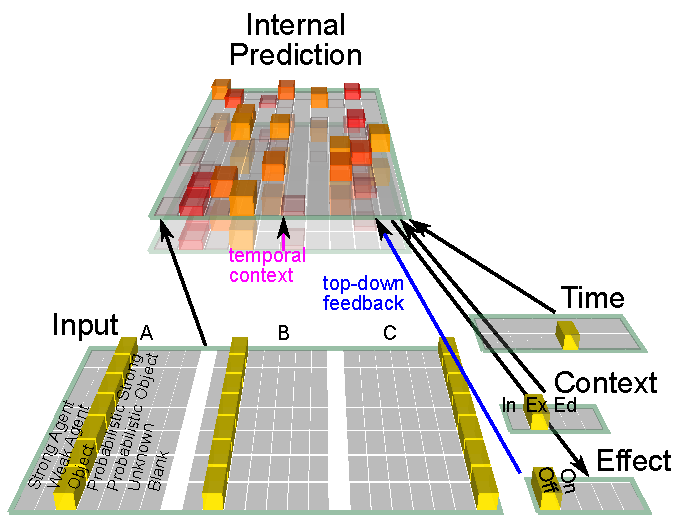
\includegraphics[width=3in]{figs/fig_blicket_net}
  \caption{\small The LeabraTI causal inference network.  Entities in the environment are encoded through 3 input channels, which represent high-level semantic representations that distinguish between inputs that are likely to be causal agents (e.g., people), weak agents that require multiple such agents to effect an outcome, and objects that are unlikely to be causal agents.  Noisy versions of agents and objects are also encoded.  For testing in the blicket-like tasks, the inputs activate the {\em unknown} category, and their causal status must be inferred as a result of the pattern of {\em Effect} activations over time, which feed back via bidirectional connections to the internal prediction layer to shape its representations.  This internal layer also has the deep cortical temporal context layer, which enables this information to be integrated over time.  The Time and Context inputs reflect the structure of the task, and are useful for visualization and decoding, but do not affect network behavior significantly.}
  \label{fig.net}
\end{figure}

The LeabraTI causal inference model (Figure~\ref{fig.net}) is designed to provide a simple, minimalist framework for learning these causal tasks (see supplemental online material for full details).  There are three different input channels, so the network can encode up to three different objects present at a time, and each channel has high-level semantic features that distinguish between the following classes of inputs: strong agent (e.g., a person, who typically is the causal agent); weak agent (e.g., requiring multiple such agents to achieve a causal outcome); object (never a causal agent); probabilistic strong agent (a strong agent with noisy causal behavior); probabilistic object (an object that is also noisy -- sometimes appears to be causal); unknown (a novel input -- e.g., a blicket); and blank, which indicates the absence of an input in this channel.  These inputs all feed into a common internal processing and prediction layer, which has an associated temporal context layer that corresponds to the deep cortical layers in the LeabraTI framework.  The primary output of the model is a prediction, generated by this internal prediction layer, of whether there will be a causal outcome of some kind (e.g., the blicket detector going off), as a result of the inputs.  There are also context and time inputs that define the structure of an input sequence (these do not affect network performance significantly, but are useful for visualization and decoding).  A typical input sequence involves presentation of the full set of objects present in a given scene, with no effects (to give the network the relevant scene context), followed by a sequence of object / effect trials, which were repeated twice.  For example, during training, a strong agent and an object could be present, and the strong agent alone or in combination with the object causes the effect, while the object alone does not.  All possible combinations of inputs and sequences were presented during training, simulating the background experience someone would have coming into a blicket experiment.  This includes 20\% of trials that included an unknown object (which was randomly assigned with uniform probability to a causal status), so that the network gained familiarity with the meaning of these inputs.  A total of 16,000 different causal input scenes were presented during training (although network performance was already quite good after 4,000).

\begin{figure}
\centering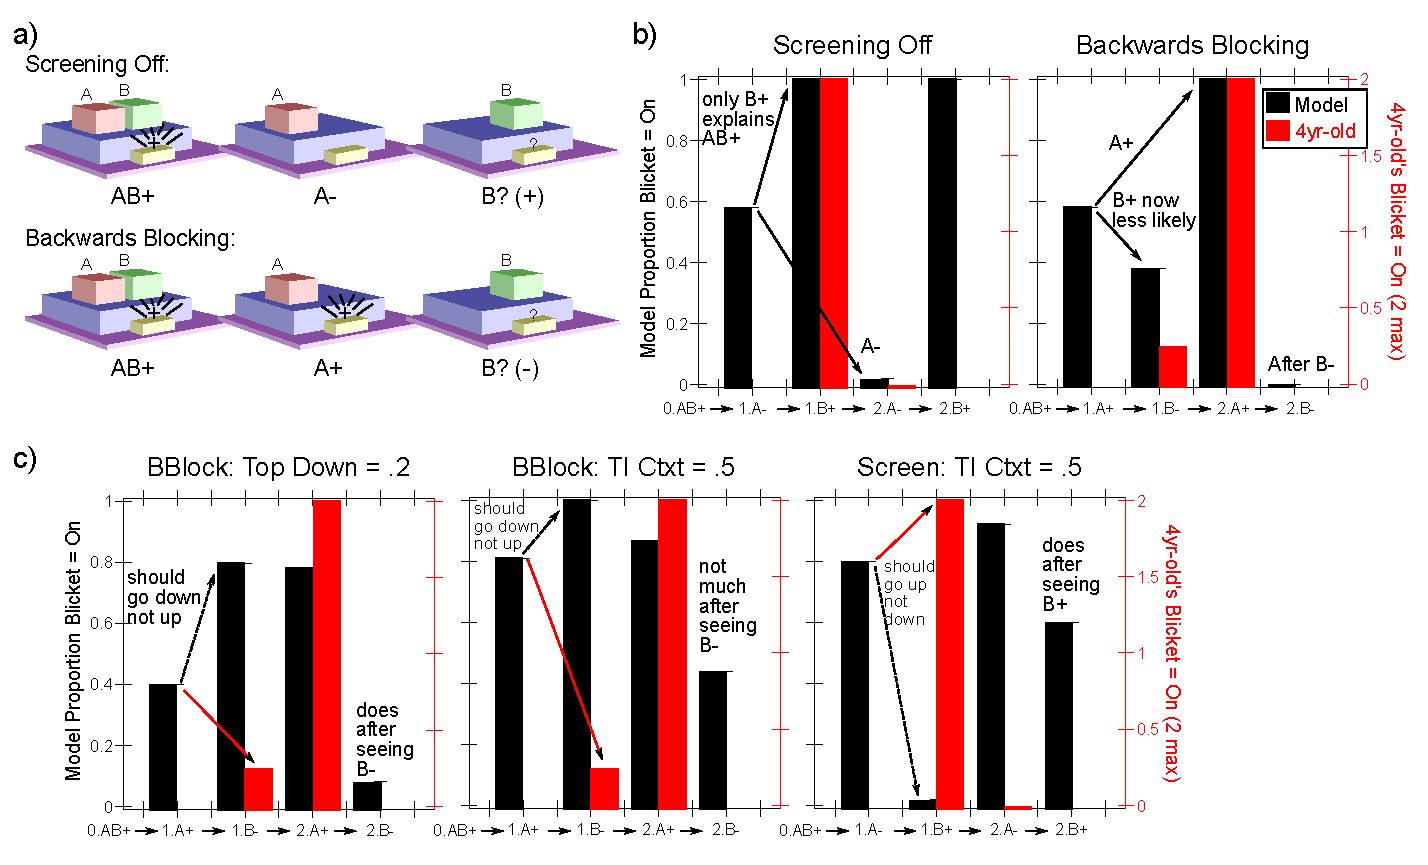
\includegraphics[width=6in]{figs/fig_blicket_stg04_bblock_all}
  \caption{\small The screening off and backwards blocking tests, and results (N=25 batches, SEM error bars too small to see).  {\bf a)} shows the two test sequences of interest.  {\bf b)} shows the average output of the Effect On unit for the two sequences, compared to 4 year-old's performance from Sobel et al., (2004).  These Effect outputs were measured in the minus phase of each trial, when the network takes its guess as to what will happen, and then it experiences the actual effect as indicated (+ = On, -- = Off).  The network is initially uncertain about the causal status of the A input, but after experiencing either the + (in blocking) or the -- (in screening off), this information feeds back and shapes the internal representations, such that it can now better expect what will happen when B alone is presented. {\bf c)} These updated predictions are not made accurately when either the top-down weight scale is reduced, or the strength of the temporal context is reduced, thus demonstrating the importance of these parameters.  Network performance is unaffected by similar increases in these parameters, as a control condition (not shown).}
  \label{fig.stg04}
\end{figure}

During testing, which followed training, only unknown inputs were presented, and the network had to infer their causal properties based on the pattern of effects across trials.  The screening off and backwards blocking conditions are illustrated in Figure~\ref{fig.stg04}, along with the results from the network in these cases, in comparison to those from 4-year-olds \cite{SobelTenenbaumGopnik04}.  These results show that the network was able to generalize its learning to these novel blicket test cases, in the same way that people do.  Specifically, when AB+ (+ indicates blicket detector going off) is followed by A-- (-- is no blicket activation), then the model correctly predicts that B alone will activate it (screening off).  Conversely, the backwards blocking case of AB+, A+, leads to a somewhat weaker inference that B alone is less likely to activate the detector.  To test for the importance of both bidirectional processing and integration of information over time, we modified these parameters in our model.  As shown in Figure~\ref{fig.stg04}c, decreasing the top-down connections from effect back to internal representation, or reducing the strength of the TI context inputs, significantly impaired performance on both the screening off and backwards blocking conditions.  Importantly, these results held whether the parameters were changed at the time of initial learning, or only at test, and only reductions, not comparable increases, led to these effects.

\begin{figure}
\centering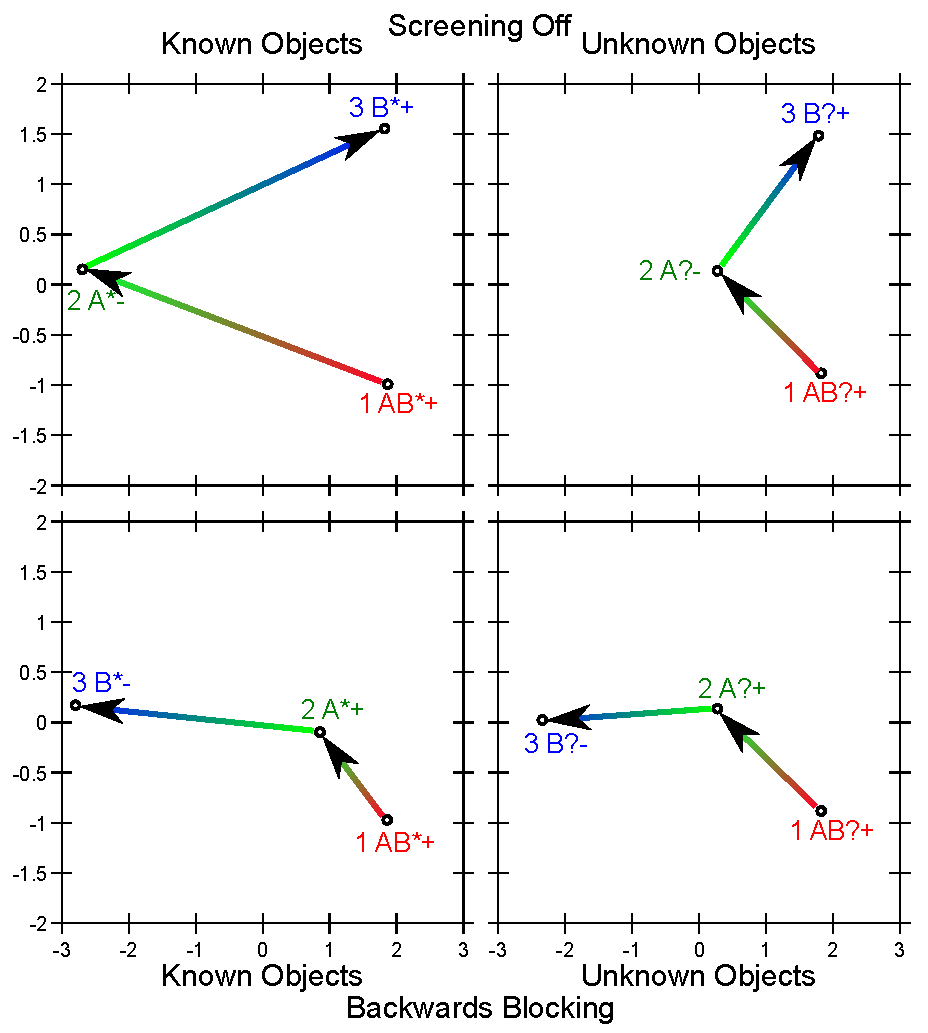
\includegraphics[width=3in]{figs/fig_blicket_pcatraj}
  \caption{\small Trajectories of the minus (prediction) state of the internal representation layer in the model over the screening off and backwards blocking sequences, using PCA to reduce to a 2 dimensional projection along the principal eigenvectors.  The pattern for known objects (where the input explicitly represents their causal status, indicated by a * in the labels) is shown on the left, for comparison against the same conditions with unknown objects on the right (where causal status must be inferred through feedback from Effect outcomes, indicated by a ?).  All cases start off in the same part of representational space for the AB inputs, but for the screening off case (top row), the network represents the unknown A? (top right) in the same way it does for the known A*+ (bottom left).  After it experiences the -- outcome for A, the representation of B is systematically shifted to coincide with the B*+ known case.  This is due to top-down feedback from the Effect output shaping the internal representation layer -- here we can see the network effectively ``thinking'': {\em A didn't activate it, so it must be B}.  A similar dynamic occurs in the backwards blocking case, and it is clear that the network assigns very different representations to B based on the prior Effect outcome for A.}
  \label{fig.pcatraj}
\end{figure}

We can examine the representations learned in the network to discover how the network accomplishes this systematic form of inference.  Figure~\ref{fig.pcatraj} plots the internal representation activations projected down to a 2 dimensional space through principal components analysis (PCA) on the activation patterns over time.  This captures the primary dimensions of variability in these patterns, and shows how the initially ambiguous input patterns come to be represented similarly to causal agents or non-causal objects depending on the pattern of causal outcomes over time.  These causal outcomes feed back into the internal representation layer, and thereby shape the evolution of the representation patterns.  This is how the recurrent or bidirectional processing feature of our models (and by hypothesis, the brain) plays such a central role in the flexible generalization of causal inferences to novel situations.

\begin{figure}
  \centering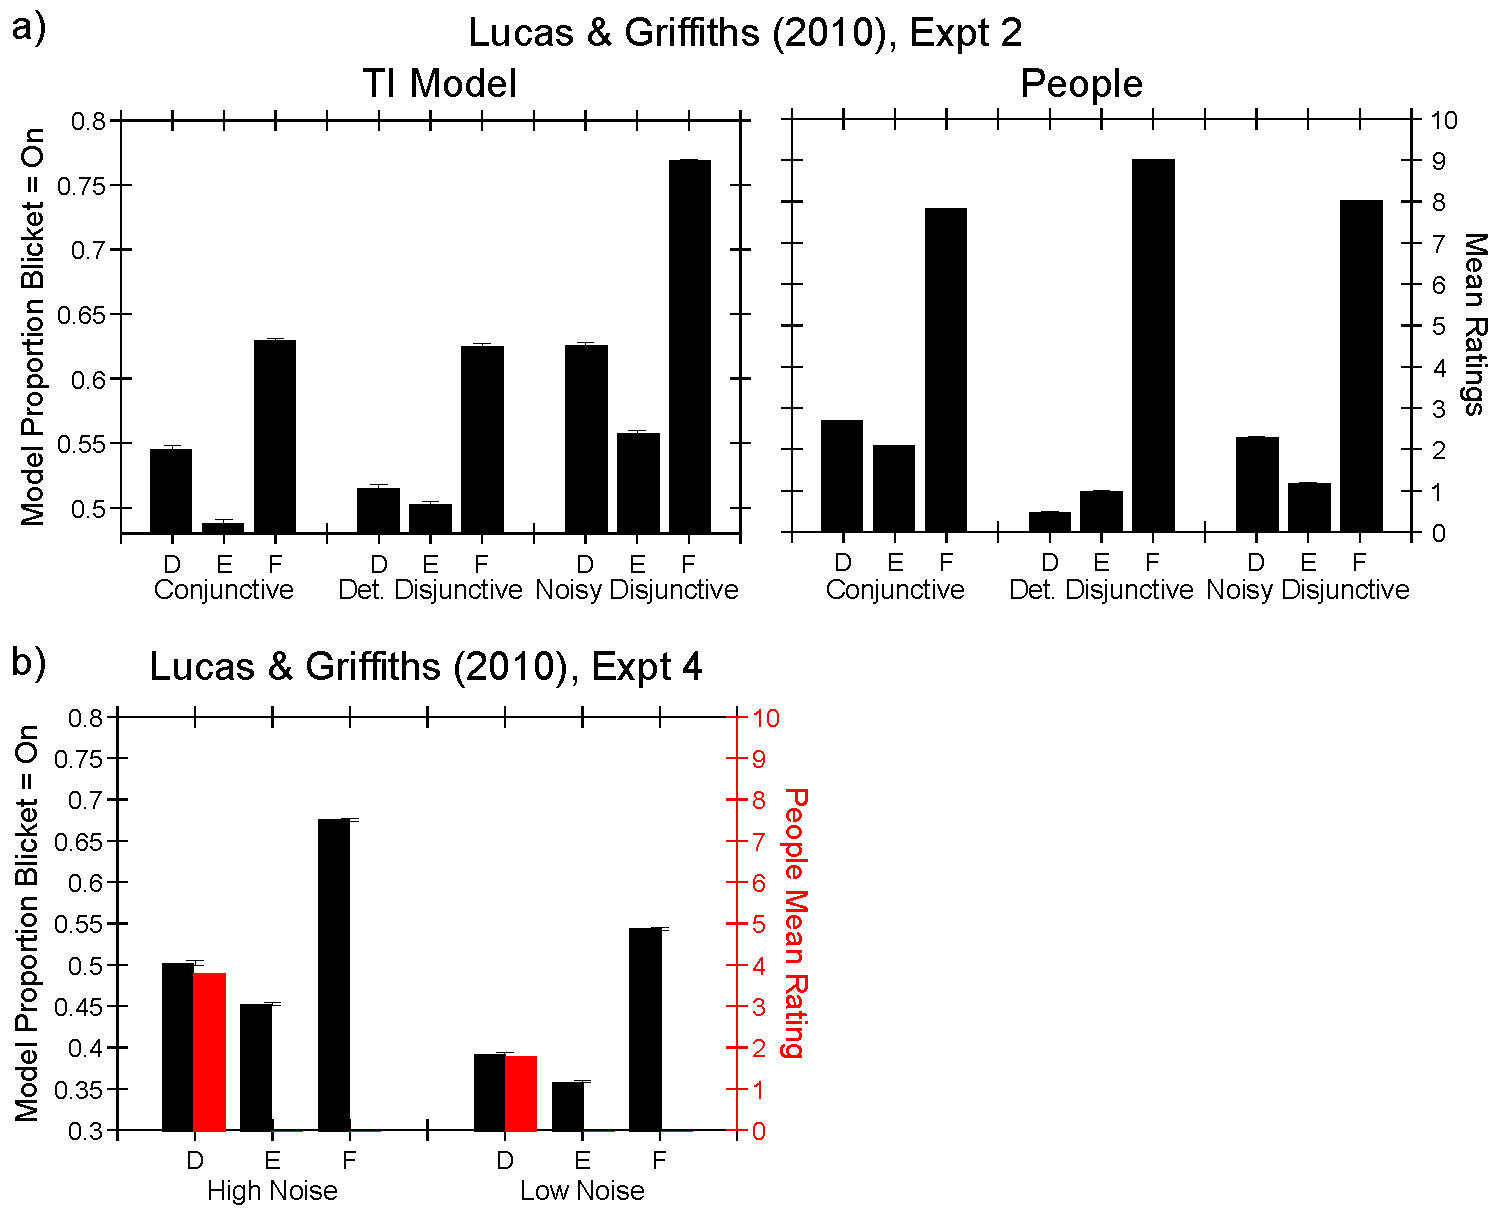
\includegraphics[width=6in]{figs/fig_blicket_lg10_all}
  \caption{\small Simulation of Lucas \& Griffiths (2010) experiments 2 and 4, showing how different prior training conditions affect responses to a common ambiguous test probe.  {\bf a)} Conjunctive: A--, B--, C--, AB--, AC+, BC-- (infer that A and C must work together); Deterministic Disjunctive: A+, B--, C--, AB+, AC+, BC-- (infer that A acts alone);  Noisy Disjunctive: A+, B--, C--, AB--, AC+, BC-- (infer that A acts alone, most of the time); Test probe is: D--, D--, D--, E--, DF+, DF+ (F more likely than others, D could be conjunctive or not depending on bias).  The model captures the qualitative patterns accurately: F always higher than others, and D higher for conjunctive than disjunctive, only for deterministic case.  E is not very relevant, and the noisy disjunctive case is a bit strange and not very diagnostic in people or the model.  {\bf b)} Low noise: A+, A+, A+, A--, A+, A+, B--, C--, AB--, AC+, BC--; High noise: A--, A--, A--, A+, A--, A--, B--, C--, AB--, AC+, BC--.  Again, model shows that these noise manipulations have appropriate effects on inferences.}
  \label{fig.lg10}
\end{figure}

Finally, Figure~\ref{fig.lg10} shows the results from our simulation of \cite{LucasGriffiths10}, which systematically manipulates the pattern of causal evidence presented to subjects prior to giving them a common ambiguous test probe.  They observed systematic, sensible effects of these manipulations, indicating that adult subjects were able to adapt their causal expectations rapidly.  The very same model we used to simulate the blicket task was also capable of exhibiting this rapid adaptation, based on the same dynamic updating of the internal representation in response to a temporal pattern of observed Effect outcomes.  This model was trained on randomly generated versions of the kinds of event sequences used in the experiment, and all tests were done on unknown inputs.  Thus, the model was able to extract the patterns associated with weak (conjunctive) and strong (disjunctive) agents, and when the prior exposure biased it into one or the other of these patterns, it generalized this pattern to subsequent ambiguous inputs.  Similarly, it was capable of generalizing prior levels of noise to the novel test case as well.

These impressive forms of generalization can be understood in more familiar terms, if we think in terms of spatiotemporally defined categories learned over temporally extended patterns --- just as abstracted categorical representations over static patterns support generalization to novel such input exemplars, so do these spatiotemporal categories.  Our model was able to induce these categorical representations from specific patterns over experience, instead of having them defined in advance by the modeler, representing an advance over existing Bayesian models, and suggesting that people could be relying on similar learning mechanisms (see \cite{OReillyWyatteRohrlichIP} for extensive additional biological and behavioral data).  Furthermore, as emphasized, this model points to the importance of bidirectional activation dynamics, which are largely missing in most current machine learning and deep network models, for supporting more complex forms of structured relational processing and inference.  In future work, we plan to explore how such learning mechanisms could also potentially explain the well-documented failures of human causal reasoning, such as our pervasive bias to infer causality from correlation, and neglect of base rates.

\bibliographystyle{Science}
%\bibliography{ccnlab}

\begin{thebibliography}{10}

\bibitem{GriffithsChaterKempEtAl10}
T.~L. Griffiths, N.~Chater, C.~Kemp, A.~Perfors, J.~B. Tenenbaum, {\it Trends
  in cognitive sciences\/} {\bf 14}, 357 (2010).

\bibitem{CiresanMeierGambardellaEtAl10}
D.~C. Ciresan, U.~Meier, L.~M. Gambardella, J.~Schmidhuber, {\it Neural
  Computation\/} {\bf 22}, 3207 (2010).

\bibitem{CiresanMeierSchmidhuber12}
D.~Ciresan, U.~Meier, J.~Schmidhuber, {\it IEEE Conf. on Computer Vision and
  Pattern Recognition CVPR 2012\/} pp. 3642--3649 (2012).

\bibitem{KrizhevskySutskeverHinton12}
A.~Krizhevsky, I.~Sutskever, G.~E. Hinton, {\it Advances in Neural Information
  Processing Systems\/} (2012), pp. 1097--1105.

\bibitem{BengioCourvilleVincent13}
Y.~Bengio, A.~Courville, P.~Vincent, {\it IEEE Transactions on Pattern Analysis
  and Machine Intelligence\/} {\bf 35}, 1798 (2013).

\bibitem{RiesenhuberPoggio02}
M.~Riesenhuber, T.~Poggio, {\it Current Opinion in Neurobiology\/} {\bf 12},
  162 (2002).

\bibitem{OReillyWyatteHerdEtAl13}
R.~C. O'Reilly, D.~Wyatte, S.~Herd, B.~Mingus, D.~J. Jilk, {\it Frontiers in
  Psychology\/} {\bf 4} (2013).

\bibitem{OReillyWyatteRohrlichIP}
R.~C. O'Reilly, D.~Wyatte, J.~Rohrlich, {\it Preprint at:
  http://arxiv.org/abs/1407.3432\/}  (submitted).

\bibitem{OReillyMunakataFrankEtAl12}
R.~C. O'Reilly, Y.~Munakata, M.~J. Frank, T.~E. Hazy, Contributors, {\it
  {Computational Cognitive Neuroscience}\/} (Wiki Book, 1st Edition, URL:
  \url{http://ccnbook.colorado.edu}, 2012).

\bibitem{OReillyMunakata00}
R.~C. O'Reilly, Y.~Munakata, {\it {Computational Explorations in Cognitive
  Neuroscience}: {Understanding the Mind by Simulating the Brain}\/} (The MIT
  Press, Cambridge, MA, 2000).

\bibitem{Elman90}
J.~L. Elman, {\it Cognitive Science\/} {\bf 14}, 179 (1990).

\bibitem{Elman91}
J.~L. Elman, {\it Machine Learning\/} {\bf 7}, 195 (1991).

\bibitem{Jordan89}
M.~I. Jordan, {\it Advances in Connectionist Theory: Speech\/}, J.~L. Elman,
  D.~E. Rumelhart, eds. (Lawrence Erlbaum Associates, Hillsdale, NJ, 1989).

\bibitem{GopnikSobel00}
A.~Gopnik, D.~M. Sobel, {\it Child development\/} {\bf 71}, 1205 (2000).

\bibitem{SobelTenenbaumGopnik04}
D.~M. Sobel, J.~B. Tenenbaum, A.~Gopnik, {\it Cognitive Science\/} {\bf 28},
  303 (2004).

\bibitem{LucasGriffiths10}
C.~G. Lucas, T.~L. Griffiths, {\it Cognitive Science\/} {\bf 34}, 113 (2010).

\bibitem{McClellandThompson07}
J.~L. McClelland, R.~M. Thompson, {\it Developmental Science\/} {\bf 10}, 333
  (2007).

\end{thebibliography}


\begin{scilastnote}
\item Supported by: ONR grant N00014-13-1-0067, ONR D00014-12-C-0638, and by the Intelligence Advanced Research Projects Activity (IARPA) via Department of the Interior (DOI) contract number D10PC20021. The U.S. Government is authorized to reproduce and distribute reprints for Governmental purposes notwithstanding any copyright annotation thereon. The views and conclusions contained hereon are those of the authors and should not be interpreted as necessarily representing the official policies or endorsements, either expressed or implied, of IARPA, DOI, or the U.S. Government.
\end{scilastnote}

\end{document}
